%   Filename    : chapter_4.tex 
\chapter{Results and Discussion}
This chapter presents the results of the study, including findings from data collection, along with the system's diagrams, designs, features, and the chatbot's design.

\section{Data Gathering Results}
The development process for developing TUKIB started with a comprehensive visit to the UPV RRC during the researchers' internship. This phase involved engaging with key personnel and understanding the intricacies of the center's operations. The following sections detail the key activities and information undertaken and gathered during this visit.

\subsection{Facility Tour}
During the visit, the researchers met with the center's director, administrative staff, and laboratory heads. This introduction provided valuable insights into the roles and responsibilities of various individuals and departments within the UPV RRC. Understanding these dynamics was crucial for tailoring the system to fit the institution's workflows.

The researchers were also given a guided tour, which provided an overview of various laboratories and services offered. These services include:

\begin{itemize}
	\item \textbf{Sample Processing.}The RRC provides sample processing services, essential for research and analysis.
	\item \textbf{Laboratory Equipment Rental} Various pieces of laboratory equipment are available for rent, which supports a wide range of scientific projects.
	\item \textbf{Training and Workshops.} The RRC offers training sessions on laboratory equipment, promoting user proficiency.
	\item \textbf{Facility Rental.} Spaces in the RRC like the Audio-Visual Room (AVR) and conference rooms, ideal for presentations, meetings, and events, are also available for rentals.
\end{itemize}

Each laboratory was introduced in detail, with specific equipment and services discussed in terms of their functionalities and purpose. The UPV RRC houses five (5) laboratories, namely: Biology, Microbiology, Nanotechnology, Applied Chemistry Laboratory, and Food, Feeds, and Functional Nutrition Laboratory.

\subsection{Stakeholder Identification and Engagement}
The success of workflow automation hinges on understanding the needs and expectations of its key stakeholders. These stakeholders include the RRC laboratory and administrative staff, the clients (university and student researchers and external users of the RRC facilities), the developers, and the member/s of the Computer Science Faculty guiding the project.

The researchers' interaction with the stakeholders allowed the gathering of valuable information on the existing system and the challenges that the institution faces. This feedback played a crucial role in shaping the direction of this study's system design, as it highlighted the need for automation, service tracking, and streamlined communication between stakeholders. Additionally, stakeholders were interviewed on their specific needs and pain points. These discussions led to the creation of user stories, which helped to contextualize the requirements from various perspectives. 

This in-depth exposure to the center’s operations was essential for the initial design and development phase of TUKIB, providing a strong foundation for creating a system tailored to the specific needs of the RRC.

\subsection{Scope and Limitations of the Services}
Through discussions with the RRC staff, the researchers obtained a clear picture of the scope of services provided by the institution, as well as, the limitations is faces. Some of these limitations include:

\begin{itemize}
	\item The UPV RRC has no website available to the public which presents its mission, vision, services offered, as well as, steps or guide on how to request a service, and other relevant information. This limits clients from acquiring necessary information about the center and its services. The only platform that they utilize for disseminating news, activities, and information about their services is through a Facebook page which lacks structure and organization.
	\item The staff also has difficulty in managing and tracking equipment and facility availability in real-time, as it is essential to ensure seamless delivery of the institution's services.
	\item Manual service request and data management are also a problem as the RRC’s current system relies mainly on Google Forms and Sheets, which poses challenges in efficiency.
\end{itemize}

\subsection{System Requirements}

Based on the gathered data with stakeholders and observations during the facility tour, several key user requirements were identified for the development of TUKIB. 

\begin{itemize}
	\item \textbf{Service Information Accessibility}
	
	A website that allows clients or researchers to gain information about the UPV RRC and the services it provides, along with the steps on how to avail those services. 
	
	\item \textbf{Automated Service Requests}
	
	A system that automates the end-to-end flow of service request process, from submission of request to giving of feedback, in order to reduce the workload on staff and provide ease for clients.
	
	\item \textbf{Equipment and Facility Availability Tracking}
	
	A system that automates the tracking of the availability of equipment and facilities. This includes a calendar that tracks the facility availability schedule and an equipment inventory management system. 
	
	\item \textbf{Data Management and Reporting}
	
	A system for managing data related to client transactions, service requests, equipment use, and facility bookings. This system should support generating detailed reports for monitoring and decision-making.
	
	\item \textbf{User Account Management}
	
	A system to monitor client profiles and their transaction history with the UPV RRC, including payments, requests, and feedbacks.
	
	\item \textbf{Feedback Mechanism}
	A feedback mechanism that allows clients to complete a service feedback survey and automatically generate feedback statistics for easier feedback analysis.
	
\end{itemize}

With the data gathered, a checklist for all the features to be implemented was made. The purpose of this was to track and verify each feature during development and testing. Table~\ref{tab:requirements} lists down all the requirements and whether these requirements have been developed and achieved.

\newpage

\begin{table}[ht]
	\centering
	\begin{tabular}{|p{10cm}|c|}
		\hline
		\textbf{Requirements/Modules} & \textbf{Accomplished (Y/N)} \\
			\hline
			\multicolumn{2}{|l|}{\textbf{Backend Requirements}} \\
				\hline
				Local Database & \\
				Automatic archiving & \\
				RESTful API & \\
				Role-based access control & \\
				Error handling, validation, \& logging & \\
				\hline
			\multicolumn{2}{|l|}{\textbf{Privacy Requirements}} \\
				\hline
				User password encryption & \\
				Session or token authentication & \\
				Restriction of unauthorized access & \\
				\hline
			\multicolumn{2}{|l|}{\textbf{User Interface Requirements}} \\
				\hline
				Client interface & \\
				Admin Staff interface & \\
				University Researcher interface & \\
				TECD Staff interface & \\
				Director interface & \\
				\hline
			\multicolumn{2}{|l|}{\textbf{Functional Requirements}} \\
				\hline
				User registration and authentication & \\
				Request tracking and management & \\
				Feedback mechanism & \\
				Notification system & \\
				Chatbot for FAQs and initial consultation & \\
				End-to-end flow of service request process & \\
				\hline
			\multicolumn{2}{|l|}{\textbf{UI/UX Design Requirements}} \\
				\hline
				Responsive design & \\
				User-friendly navigation & \\
				Feedback/confirmation messages & \\
				\hline
	\end{tabular}
	\caption{System Requirements Checklist}
	\label{tab:requirements}
\end{table}

\section{System Design}

\subsection{Process Flow Diagram}

\figref{fig:process_flow} illustrates the complete service delivery process of the UPV RRC through TUKIB. The process begins with a service request from the client and proceeds through multiple stages, including review and approval, and execution of the service. The process concludes with collecting a feedback from the client, providing opportunities for continuous improvement.

\begin{figure}[h]
	\centering 
	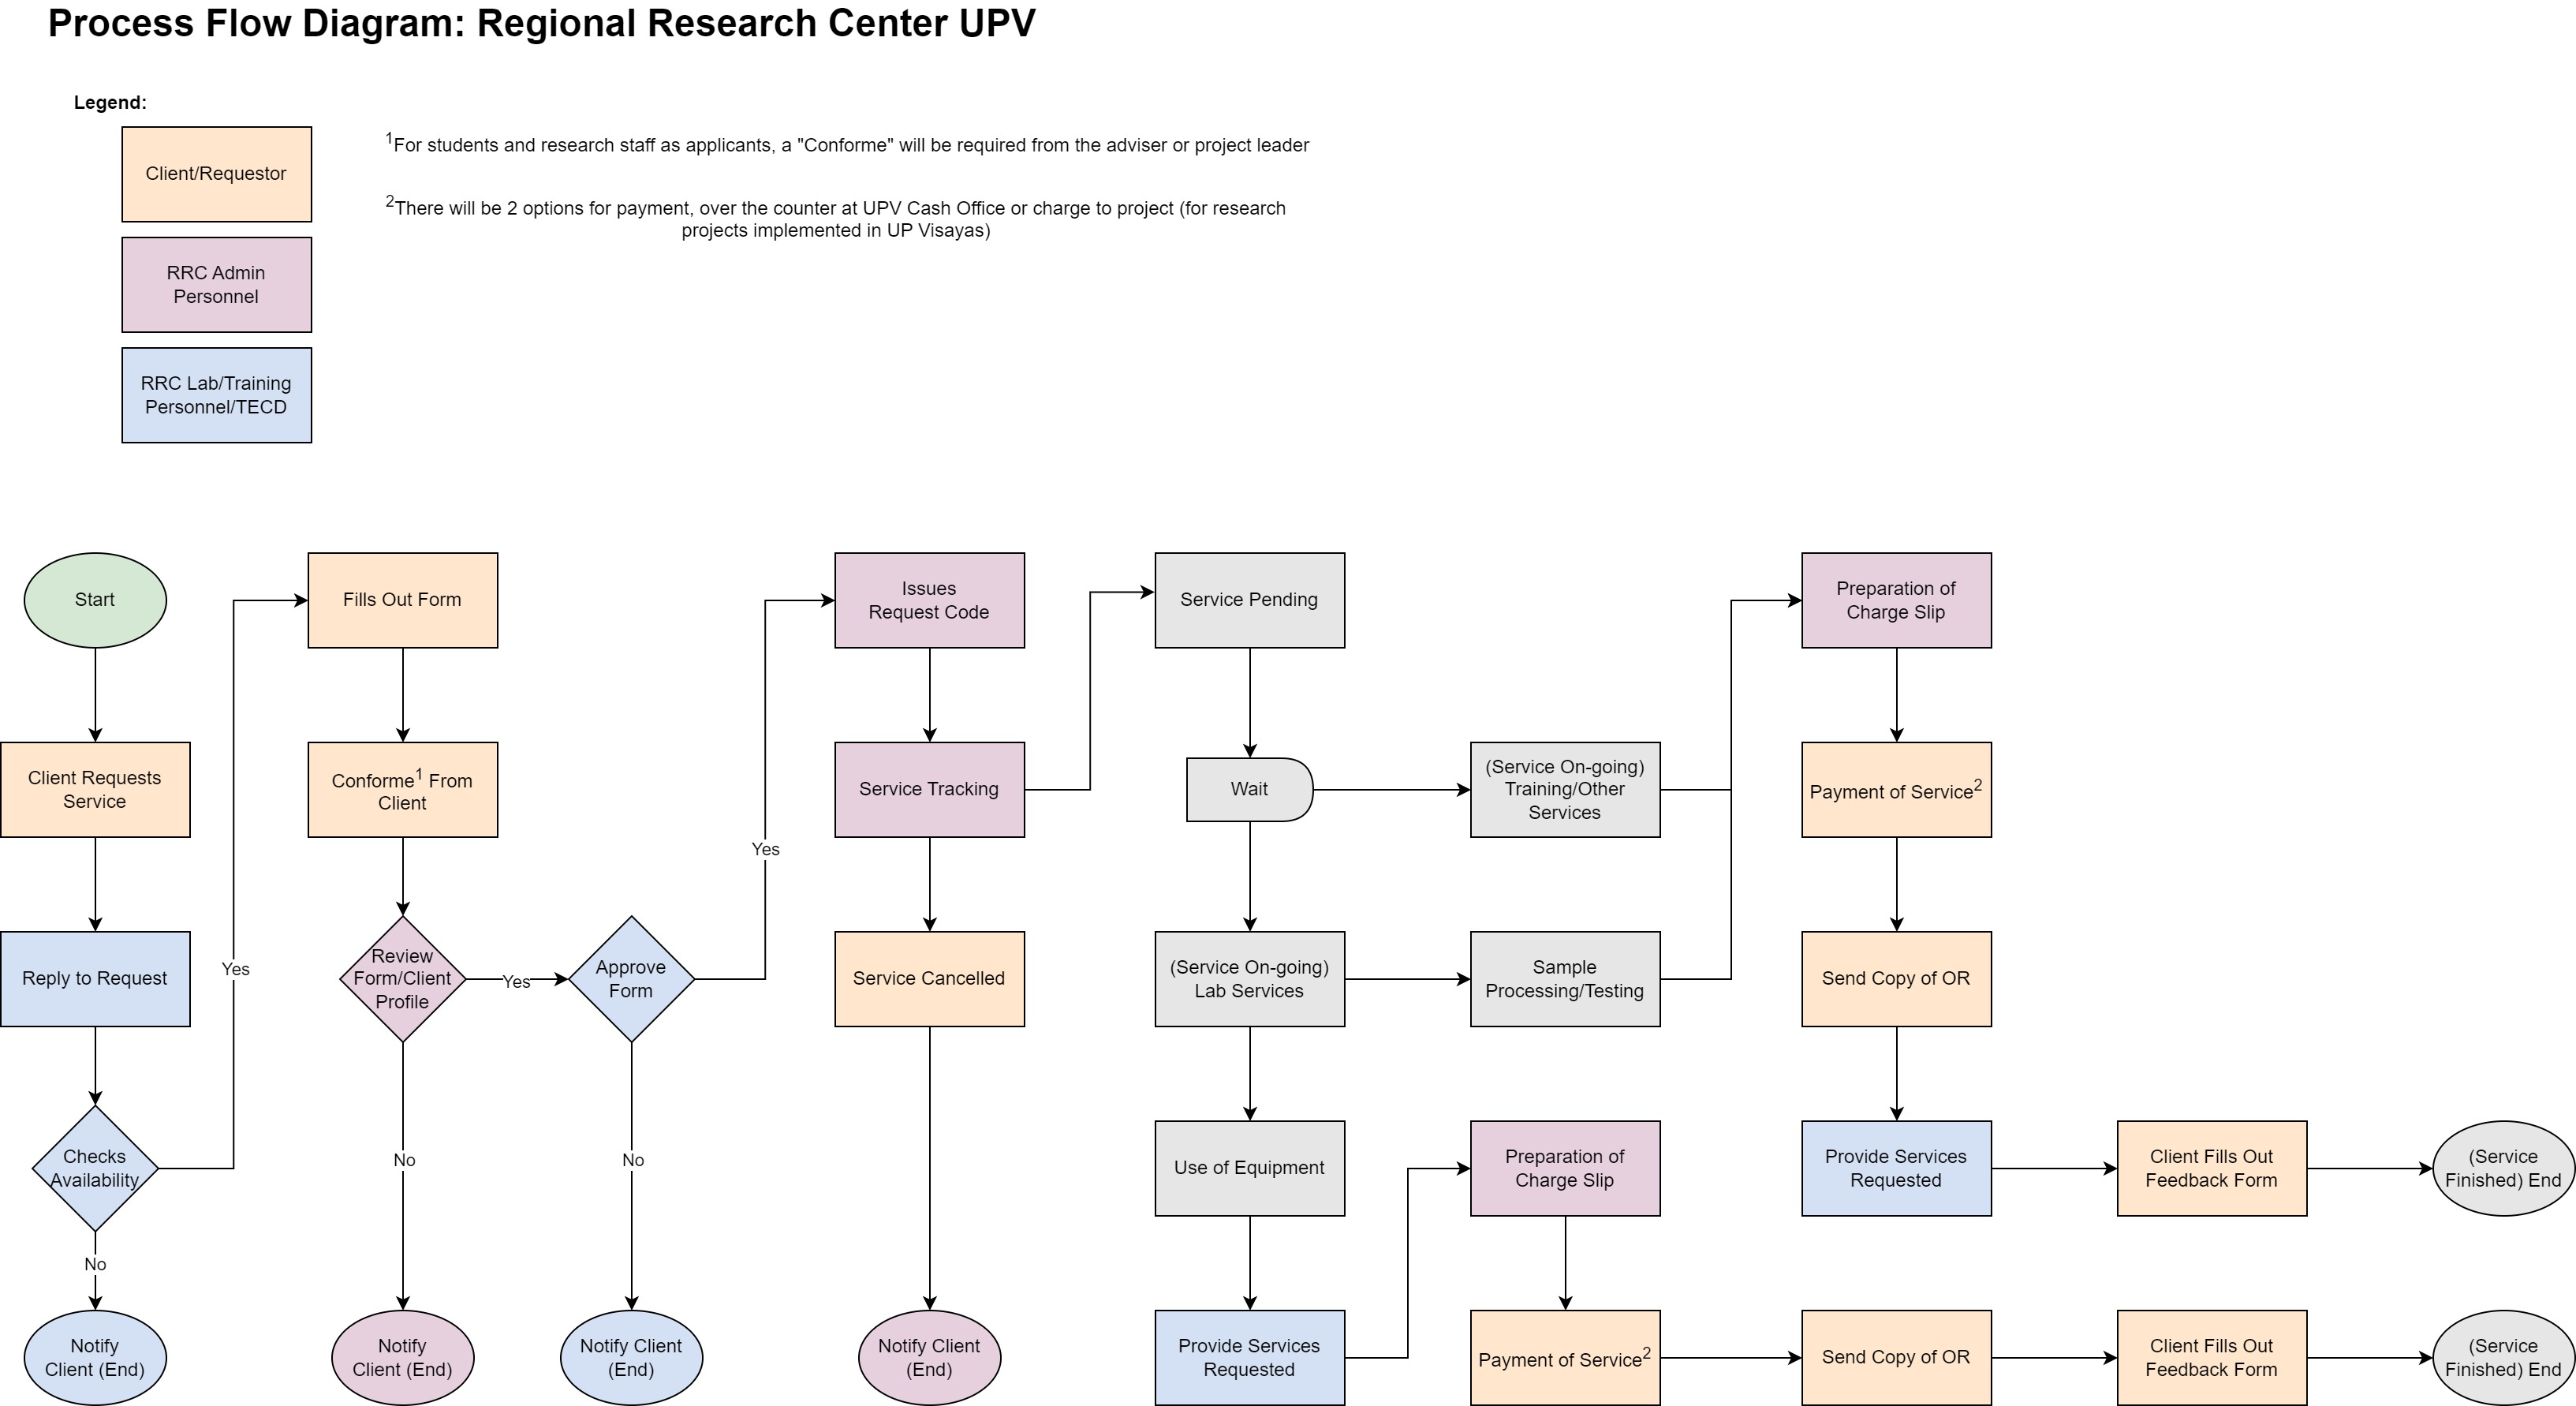
\includegraphics[width=1\textwidth]{process_flow.jpg}
	\caption{Process Flow Diagram}
	\label{fig:process_flow}
\end{figure}

\newpage

\subsection{Context Model}

\figref{fig:context_model} illustrates the interactions between the system and both internal and external entities. It shows how the system communicates with different stakeholders, including client, staff, director, and university researcher. The model also outlines how information flows from entities to the system and vice versa, showing how it works and its role within the institution.

\textbf{Clients} will primarily interact with the system to make service inquiries or submit requests related to the services offered by the UPV RRC. They might also provide feedback or report issues based on their interactions with the system or their overall experience on transacting with the UPV RRC.

For the \textbf{University Researchers}, they can use the system to oversee any laboratory-related requests, such as assessing, approving and terminating requests. Additionally, they can also use the system to release the results of the service rendered, if the client wishes to have it in softcopy. 

Similarly, \textbf{TECD Staff} can use the system to oversee, equipment or facility rental related requests. This also includes assessing, approving, and terminating request. 

For the \textbf{Admin Staff}, the system will provide oversight on the ongoing transactions. Admin staff ensure that users from various roles perform their duties effectively by managing accounts, permissions, and system-wide configurations. Like the university researchers and TECD staff, they also have access on the service-related requests and have an ability to assess, approve, and terminate transactions or requests.

\newpage

Moreover, the system will provide full oversight of activities to the \textbf{Director}, offering comprehensive visibility and control. Furthermore, the Director will have access to detailed statistics and insights about the services offered, enabling the institution to make informed and strategic decisions.

\begin{figure}[h]
	\centering 
	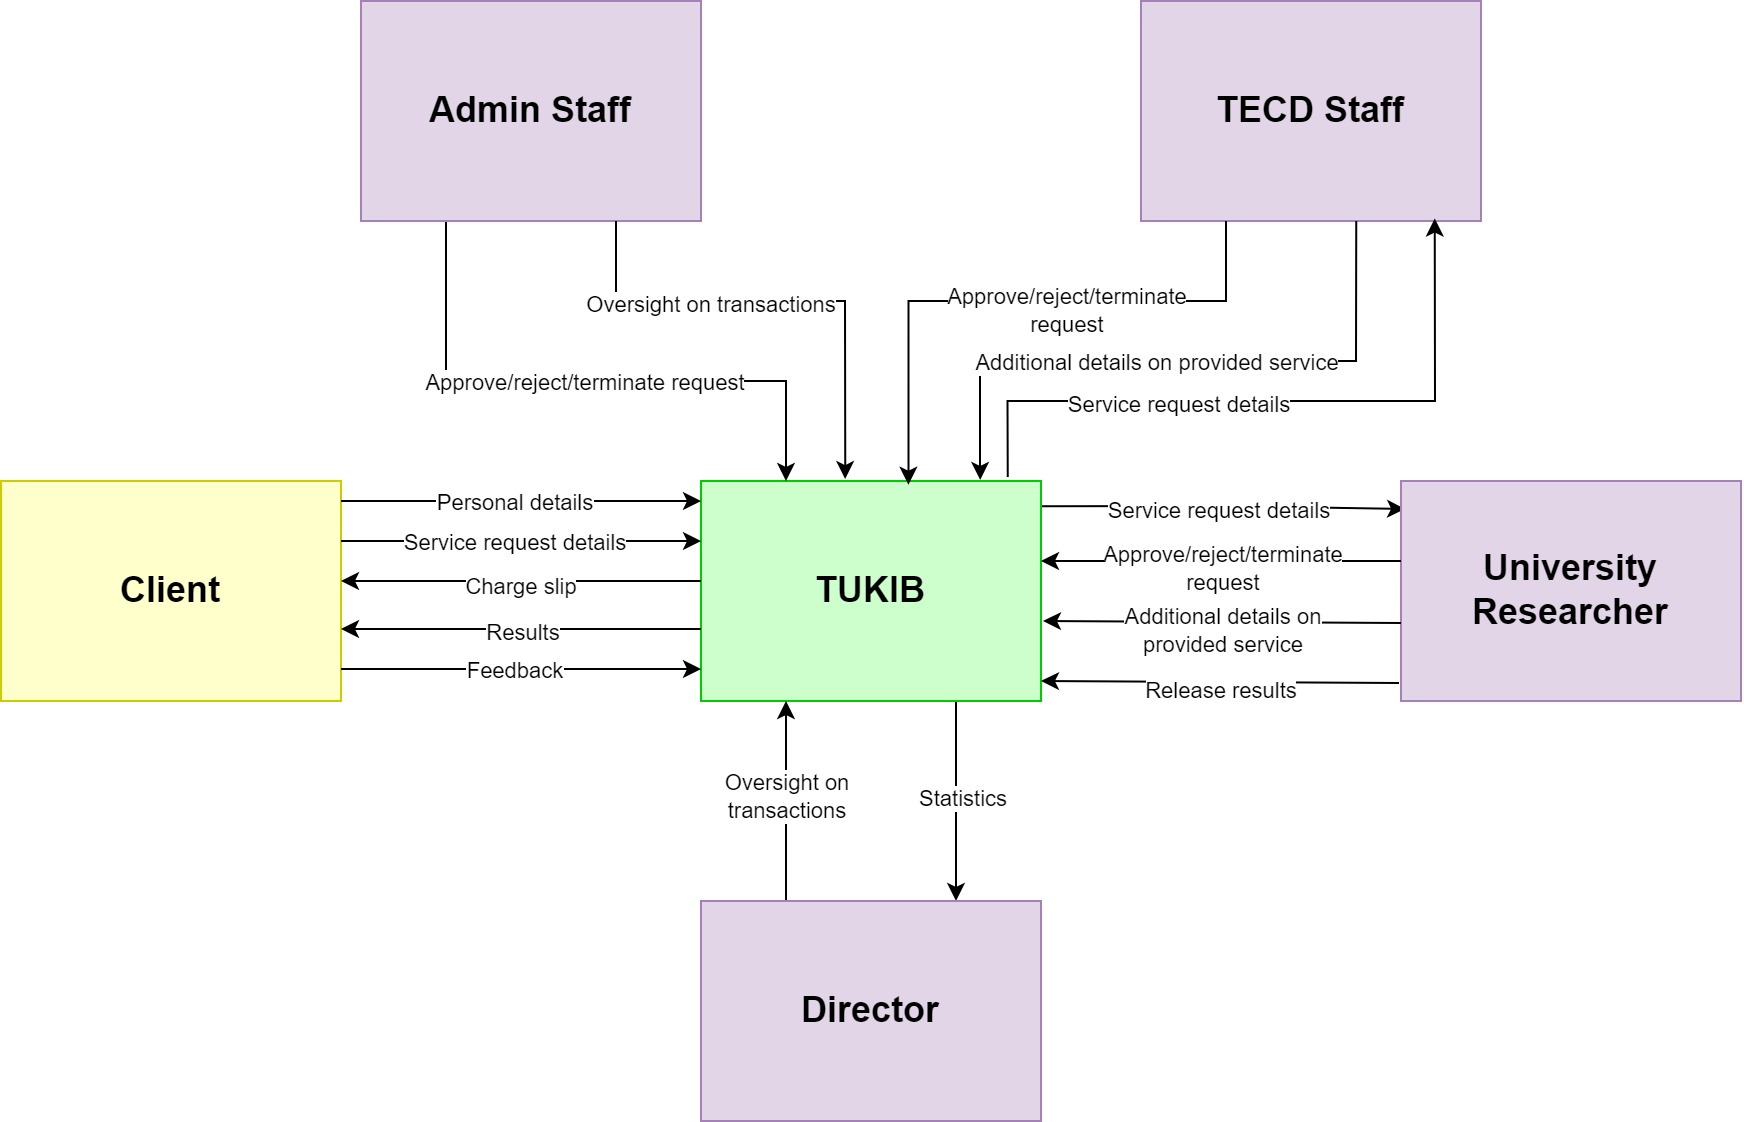
\includegraphics[width=1\textwidth]{context model.png}
	\caption{Context Model}
	\label{fig:context_model}
\end{figure}

\subsection{Use Case Diagram}

Figures \ref{fig:use_case_client}, \ref{fig:use_case_admin}, \ref{fig:use_case_director}, and \ref{fig:use_case_staff} present the use case diagrams of the system, which visually represent the key interactions between different types of users and the system in the service management cycle of the UPV RRC. The diagrams highlight the various roles and their associated tasks in managing service requests.

\newpage

\begin{figure}[h]
	\centering
	\begin{minipage}{0.30\textwidth}
		\centering
		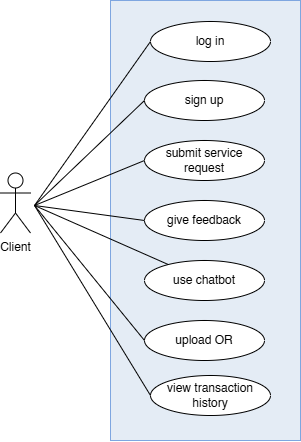
\includegraphics[width=\textwidth]{use_case_client.jpg}
		\caption{Use Case Diagram (Client interface)}
		\label{fig:use_case_client}
	\end{minipage}%
	\hfill
	\begin{minipage}{0.32\textwidth}
		\centering
		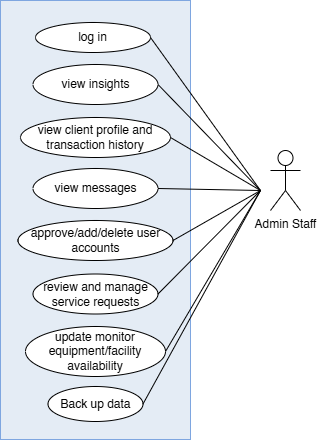
\includegraphics[width=\textwidth]{use_case_admin.jpg}
		\caption{Use Case Diagram (Admin interface)}
		\label{fig:use_case_admin}
	\end{minipage}
	
	\vspace{0.5cm} % Add some vertical space between the rows
	
	\begin{minipage}{0.30\textwidth}
		\centering
		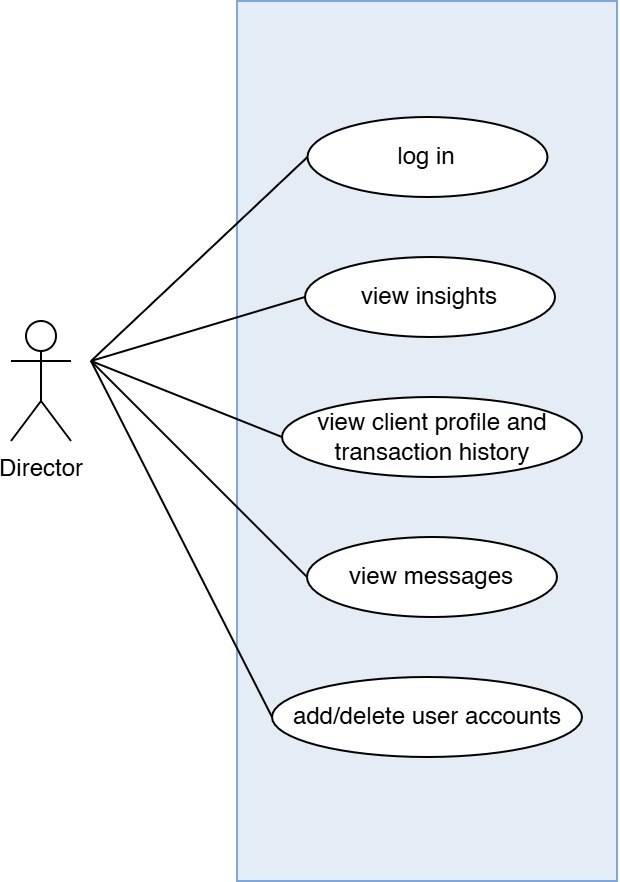
\includegraphics[width=\textwidth]{use_case_director.jpg}
		\caption{Use Case Diagram (Director interface)}
		\label{fig:use_case_director}
	\end{minipage}%
	\hfill
	\begin{minipage}{0.30\textwidth}
		\centering
		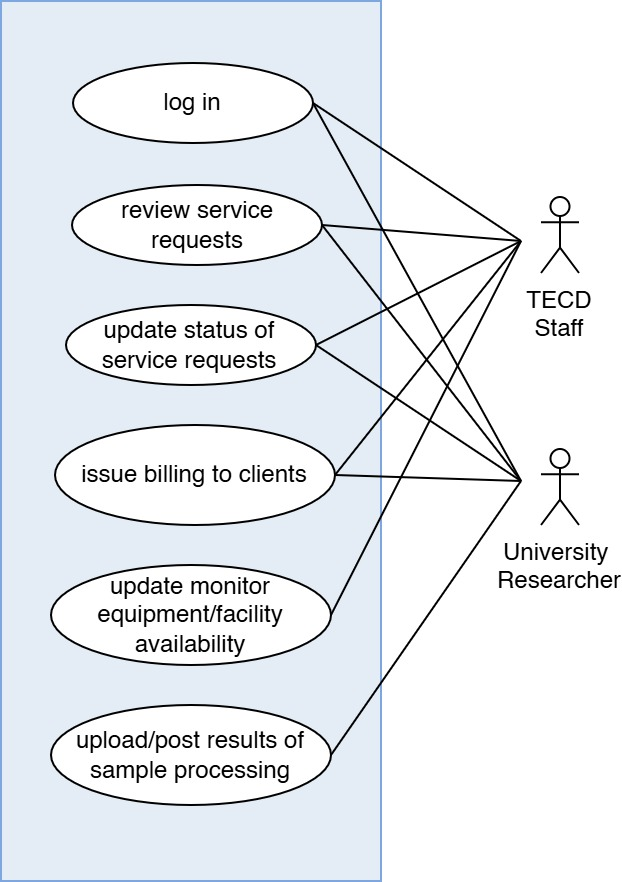
\includegraphics[width=\textwidth]{use_case_staff.jpg}
		\caption{Use Case Diagram (TECD and UR interface)}
		\label{fig:use_case_staff}
	\end{minipage}
\end{figure}

\newpage

\subsection{Data Flow Diagram}

\figref{fig:data_flow} shows the flow of data within the system, illustrating how information is exchanged between different components and users through the entire service request and delivery process of the UPV RRC. The diagram also illustrates the pathways through which data moves, providing overview into how information are stored and retrieved within the system.

\begin{figure}[h]
	\centering 
	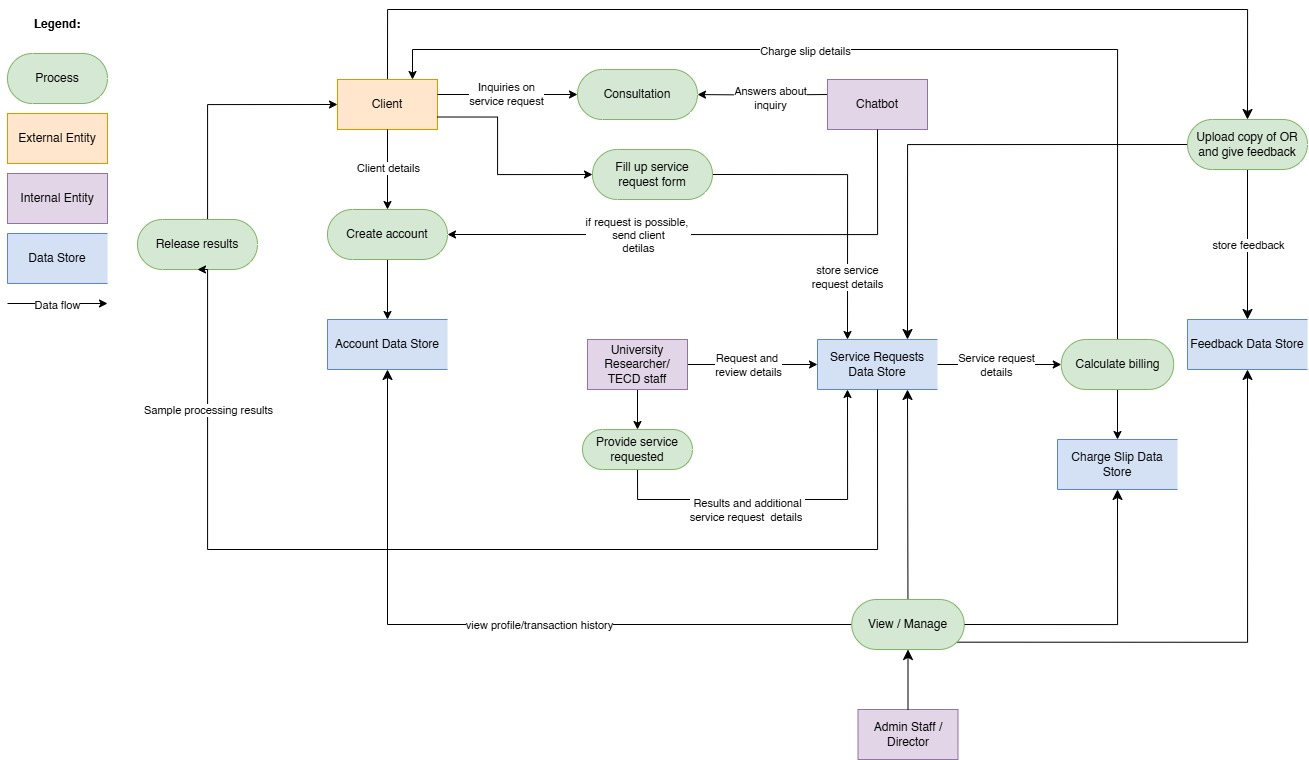
\includegraphics[width=1\textwidth]{data_flow.jpg}
	\caption{Data Flow Diagram}
	\label{fig:data_flow}
\end{figure}

\subsection{Database Diagram}

The database design for TUKIB revolves around tracking and managing various service related data through several interrelated entities to ensure easy storing and retrieval. As seen in \figref{fig:database}, there are a total of 11 tables in the database design for the TUKIB. 

The \textbf{client} table stores essential information about the clients, such as their name, contact details, and addresses. Similarly, the \textbf{staff} table also stores the necessary details of staff including name, contact details, and position. 

When a client wishes to avail a service, a corresponding \textbf{service request} is created, linking the request to both the client and the staff members handling the service. This table also records the type of service (e.g., use of equipment, use of facility, sample processing, or training) and its status. To track the usage of specific resources, there are separate tables for the \textbf{use of equipment} and \textbf{use of facility}, which log the details of which equipment or facility was used for a particular service request, including the time of use and duration. For other services, the \textbf{sample processing} table tracks the handling and status of samples, while the \textbf{training service} table records information about any training sessions provided to clients, including the assigned staff and training details. The \textbf{equipment} table stores the information about availability of equipments and history usage. 

Once the requested service is rendered, the \textbf{charge slip} table handles the relevant information needed for billing including the cost of the service. Consequently, the \textbf{payment} table ensures that all transactions are logged, tracking the payment amounts and methods linked to specific services. Additionally, feedback from clients on their experience on availing a service is stored in the \textbf{feedback} table, providing valuable insights into the service quality and client satisfaction.

\begin{figure}[h]
	\centering 
	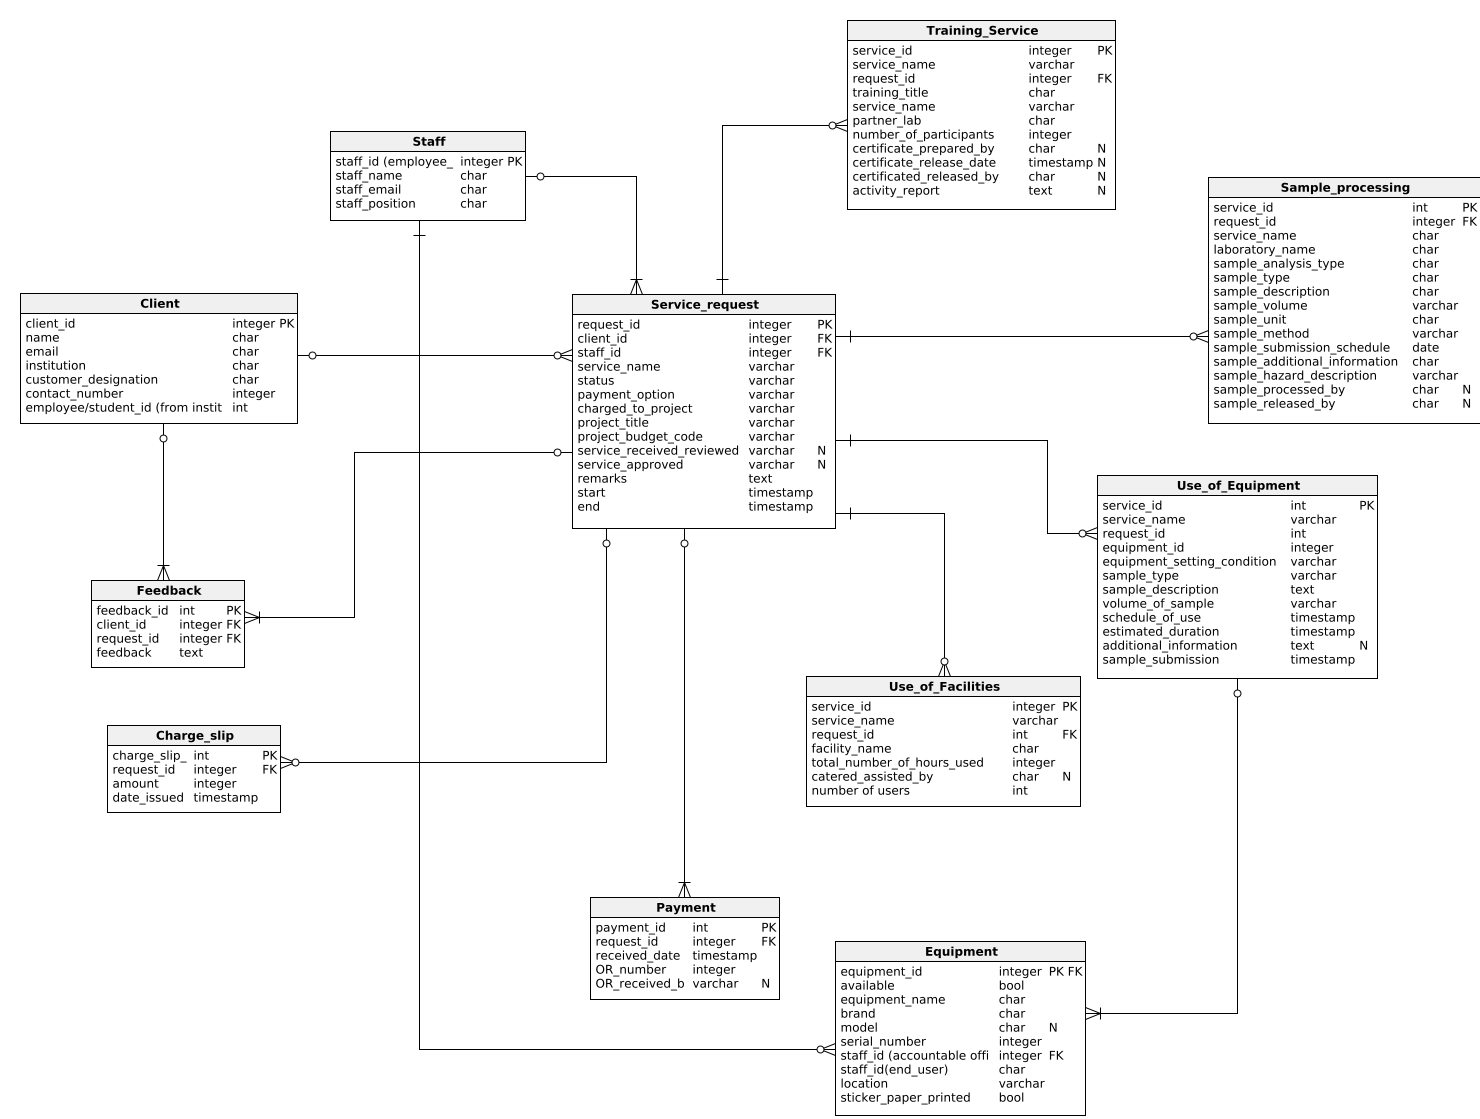
\includegraphics[width=1\textwidth]{database.png}
	\caption{Database Design Diagram}
	\label{fig:database}
\end{figure}

\newpage

\section{Chatbot}

\subsection{Entities and Intents}

From the data gathering phase, the developers were able to identify common user queries and specific service requirements needed for the development of the chatbot. The collected data was used to construct the intents and entities which are essential for the chatbot’s functionality. 

Intents represent the goal the users want to achieve when interacting with the chatbot (e.g., ”start consultation,” ”ask about lab rental procedures,” ”inquire about service status”). The intents are divided into greeting, general, service requests, frequently asked questions, feedback, and end or closing message. On the other hand, entities are specific pieces of information that the chatbot needs to get from the user in order to fulfill a task. For example, the chatbot needs to know the name of the equipment and desired time for renting in order to indicate the equipment's availability. 

\subsection{Conversation Flow}

\figref{fig:chatbot_flow} illustrates the conversation flow for TUKIB's chatbot, named LIRA— short for Learning, Innovation, and Research Assistant. LIRA will be accessible throughout the entire website, ensuring that all users, whether logged in or not, can obtain support whenever needed. Users can initiate a chat with LIRA via a persistent button that remains visible across the site or by selecting the dedicated “New Service” button found on the user dashboard.

\newpage

\begin{figure}[h]
	\centering 
	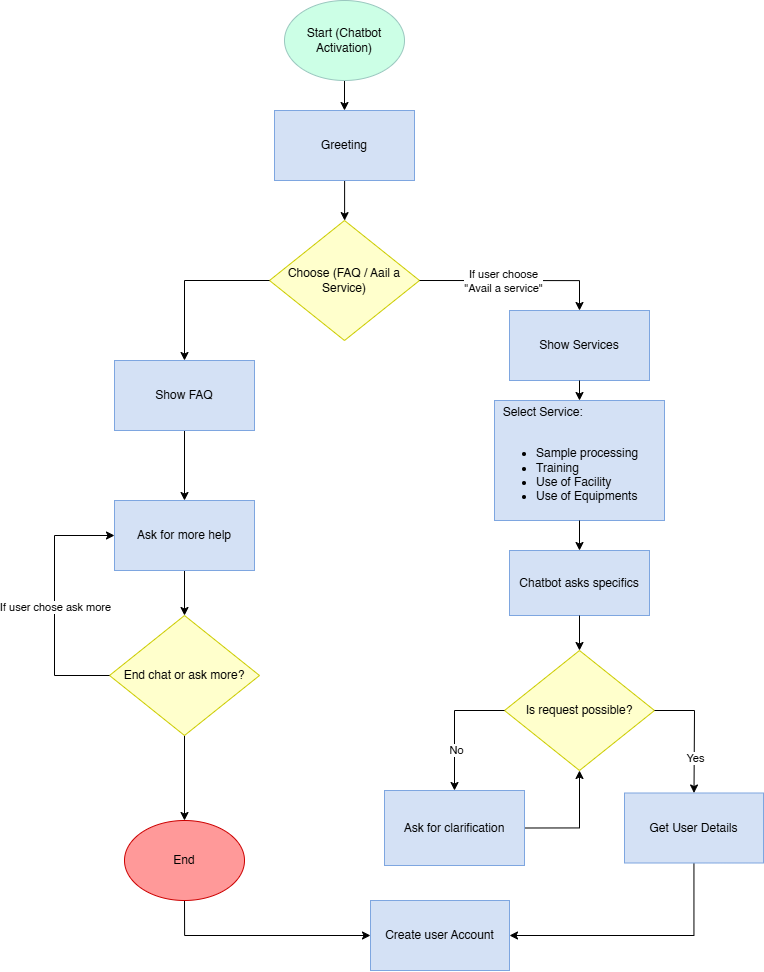
\includegraphics[width=0.7\textwidth]{chatbot_flow.png}
	\caption{LIRA Conversation Flow}
	\label{fig:chatbot_flow}
\end{figure}

\newpage

The structure of the chatbot is centered around a conversational flow that guides users through various tasks, from inquiries to service request consultations. The chatbot’s design consists of the following core components:

\begin{itemize}
	\item \textbf{Welcome Greeting}
	
	Present a welcome message where the chatbot greets users with a friendly introduction and offers assistance, presenting options such as “Service Inquiry“ and “Frequently Asked Questions/FAQs” \newline
	
	\item \textbf{Flow for Service Inquiry}
	
	If the user chooses the option “Service Inquiry,” the chatbot will ask a follow-up question to identify which service the user wishes to inquire about. Sample service choices include sample processing,  lab equipment rental, etc. Then, the chatbot uses the user's answer details to present accurate information about each service. \newline
	
	\item \textbf{Flow for Consultation}
	
	The flow for consultation is designed to facilitate user inquiries about the services they wish to avail. As the primary purpose of the chatbot, this interaction allows users to ask questions about the services offered by RRC. When a user expresses interest, the chatbot engages by asking for specific details related to their request. For instance, if a user inquires about sample processing (e.g., the type of sample and processing methods needed), the chatbot will guide them through the details. This interactive process ensures that users receive tailored information while the chatbot gathers necessary details to asses service feasibility. \newline
	
	\item \textbf{Flow for General Questions / FAQ}
	
	The chatbot should be able to answer and handle frequently asked questions by clients. These would include questions about general services, rental pricing methods, facility rental processes, etc. \newline
	
	\item \textbf{Chatbot User Feedback}
	
	Once the conversation with the chatbot is completed, it will prompt the user to rate or provide feedback on their experience, which will help the developers and the UPV RRC to in enhancing the bot and the customer satisfaction. \newline
	
	\item \textbf{Error Handling}
	
	Chatbot failures will lead to conversational dead ends if not dealt with properly. Thus, negating the main purpose of chatbot in this system which is to provide efficient customer service. To address this, the chatbot will have a fallback mechanism whenever an input from user was unexpected or a system error occurs. For example, if the chatbot cannot understand the user input, there will be rules on how the chatbot would handle this situation. Sample fallback methods would be redirecting the conversation to a live agent. Another option would be presenting friendly-toned error messages to the users, letting them know that the chatbot is having trouble understanding their input.
	 
	\subitem Sample error messages include “Sorry, I didn't catch that. Could you rephrase your question?” or “I'm sorry, I have a hard time understanding. Could you please rephrase your query?” and “I'm sorry, but what you're asking is not clear to me. Could you paraphrase it?”
	
\end{itemize}

\section{System Features}

This section elaborates the features of TUKIB. This is divided into categories different categories to cover all the features that was built throughout the development.

\subsection{Main Pages}

\noindent\textbf{Landing Page}

\figref{fig:landing} showcases the landing page of the website for the system. The page features easy navigation to essential information and pages including home, news and announcements, services, laboratories, and about. A log in button is also included on the top right of the page to ensure that user's can quickly access their accounts. Additionally, a persistent button for the chatbot is found on the bottom left of the page. 

\newpage

\begin{figure}[h]
	\centering 
	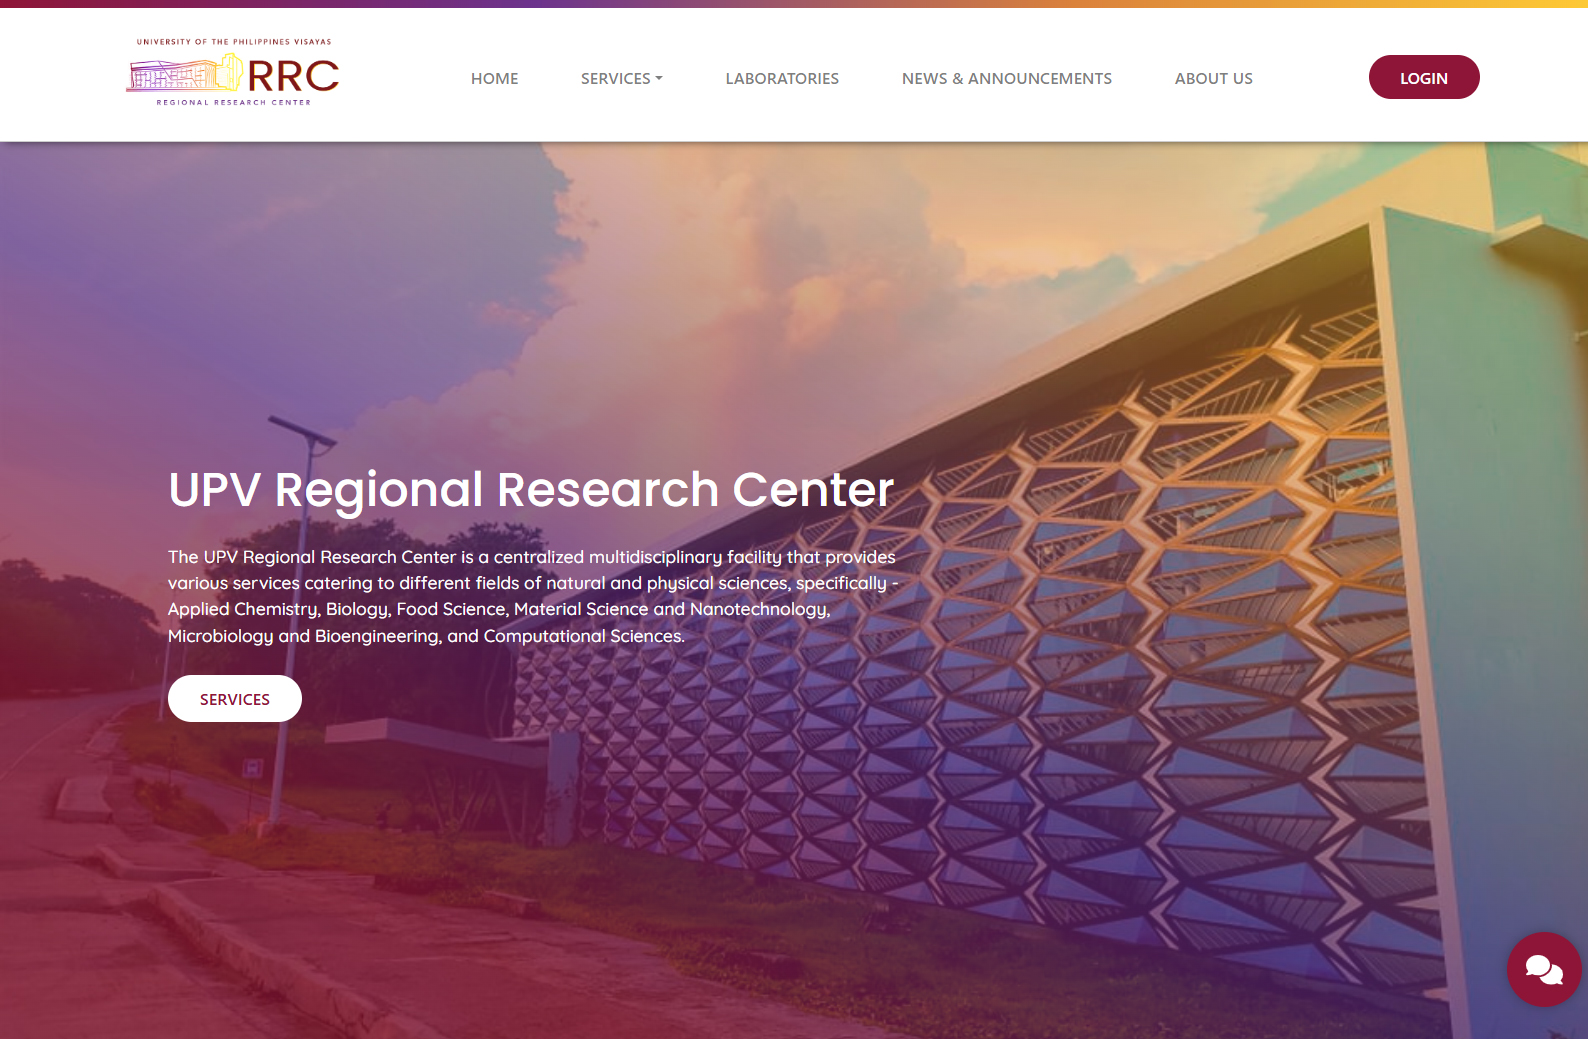
\includegraphics[width=0.8\textwidth]{landing.png}
	\caption{Landing/Homepage}
	\label{fig:landing}
\end{figure}

\noindent\textbf{Services Page}

Figure \ref{fig:service_page} shows the 'Services' page. Each service has a separate page that includes a description of the service, pricing information, and instructions or guide on how to avail the service. This structure facilitates easier navigation and helps users find the information they need efficiently.

\begin{figure}[h]
	\centering
	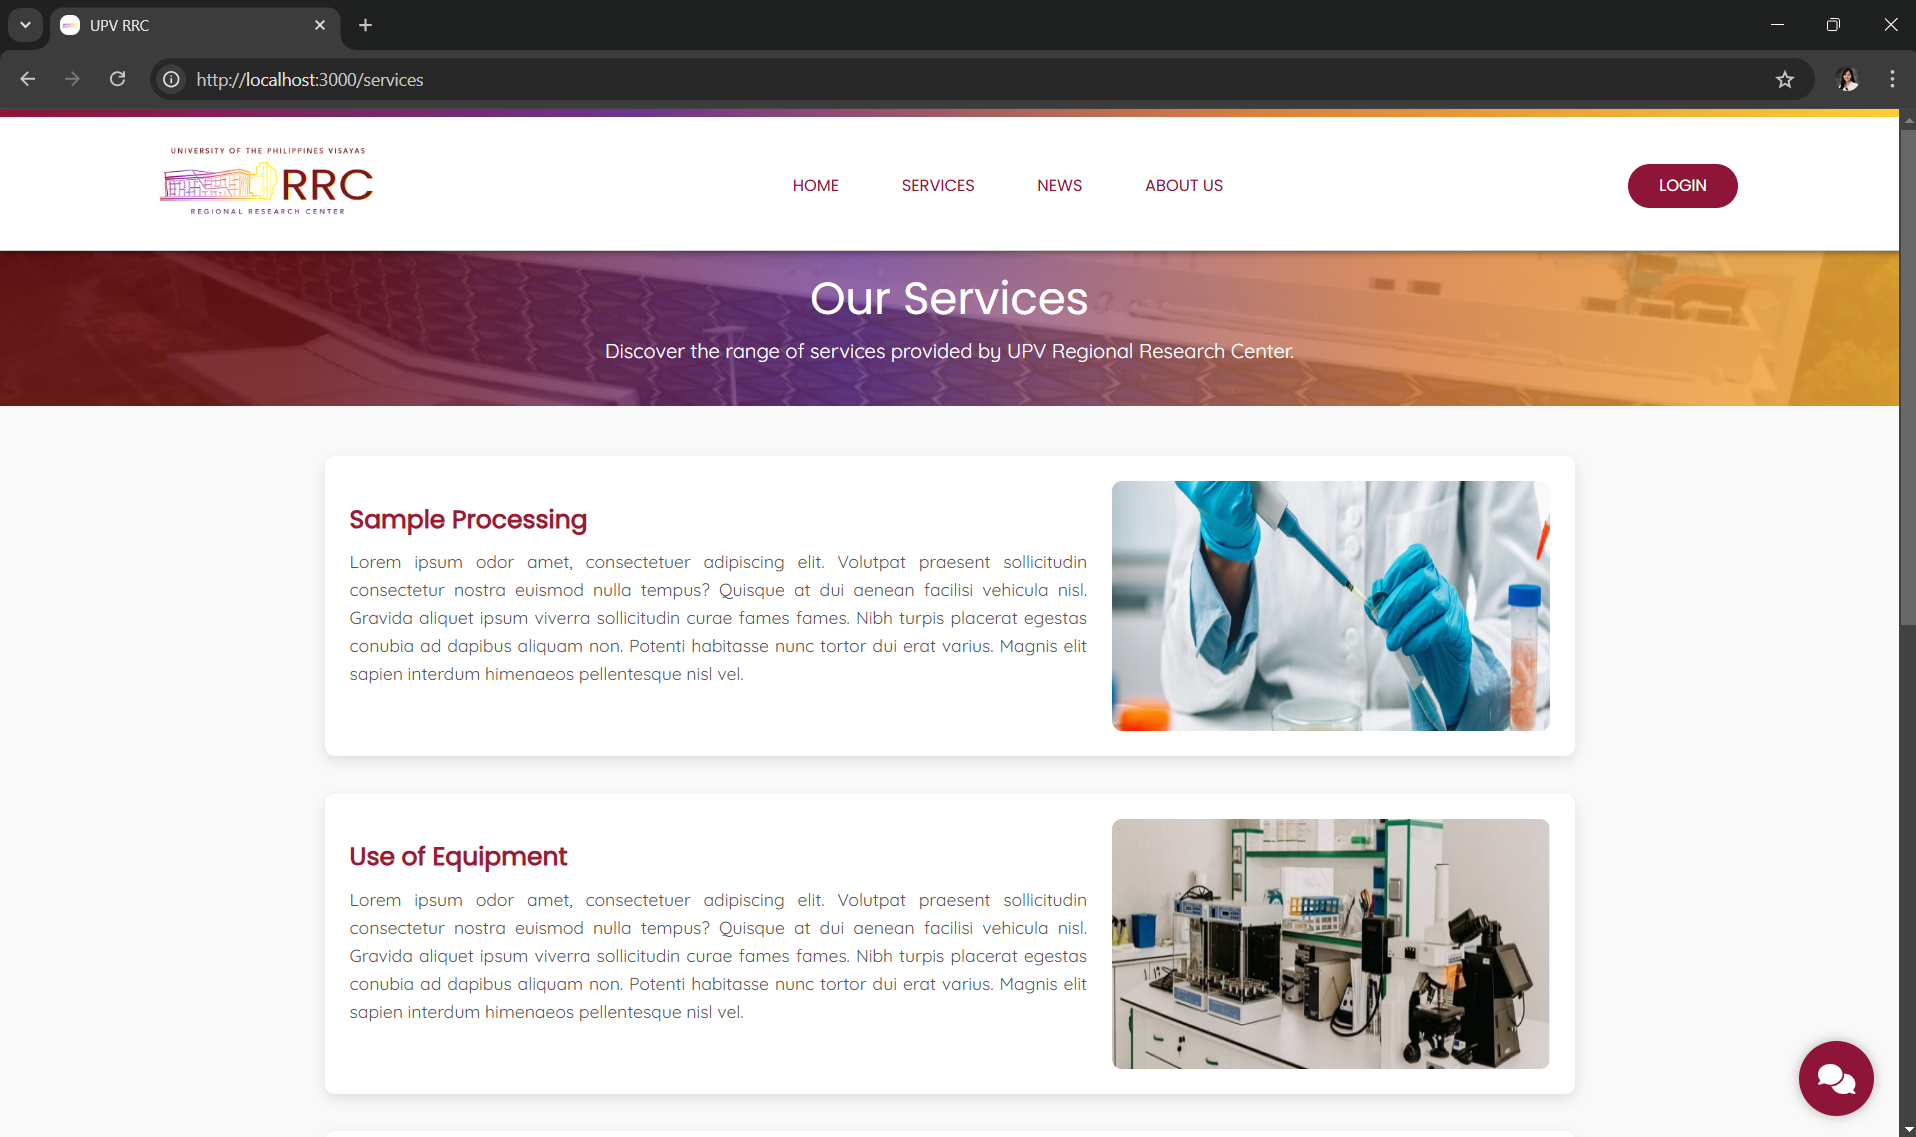
\includegraphics[width=0.8\textwidth]{service_page.png}
	\caption{Services Page}
	\label{fig:service_page}
\end{figure}

\newpage

\noindent\textbf{Laboratories Page}

Figure \ref{fig:laboratories_page} shows the 'Laboratories' page. This page displays information about the laboratories within the UPV-RRC, including the available equipment for each lab. It also provides brief descriptions of each piece of equipment to give clients a better understanding of what is available.

\begin{figure}[h]
	\centering
	
\includegraphics[width=0.8\textwidth]{laboratories.png}
	\caption{Laboratories Page}
	\label{fig:laboratories_page}
\end{figure}

\newpage

\noindent\textbf{News and Announcements Page}

Figure \ref{fig:news_page} is the 'News and Announcements' page. This page serves as the central hub for all important updates related to the UPV RRC, including news about upcoming events, recent developments, announcements of new equipment or services, and relevant research highlights.

\newpage

\begin{figure}[h]
	\centering
	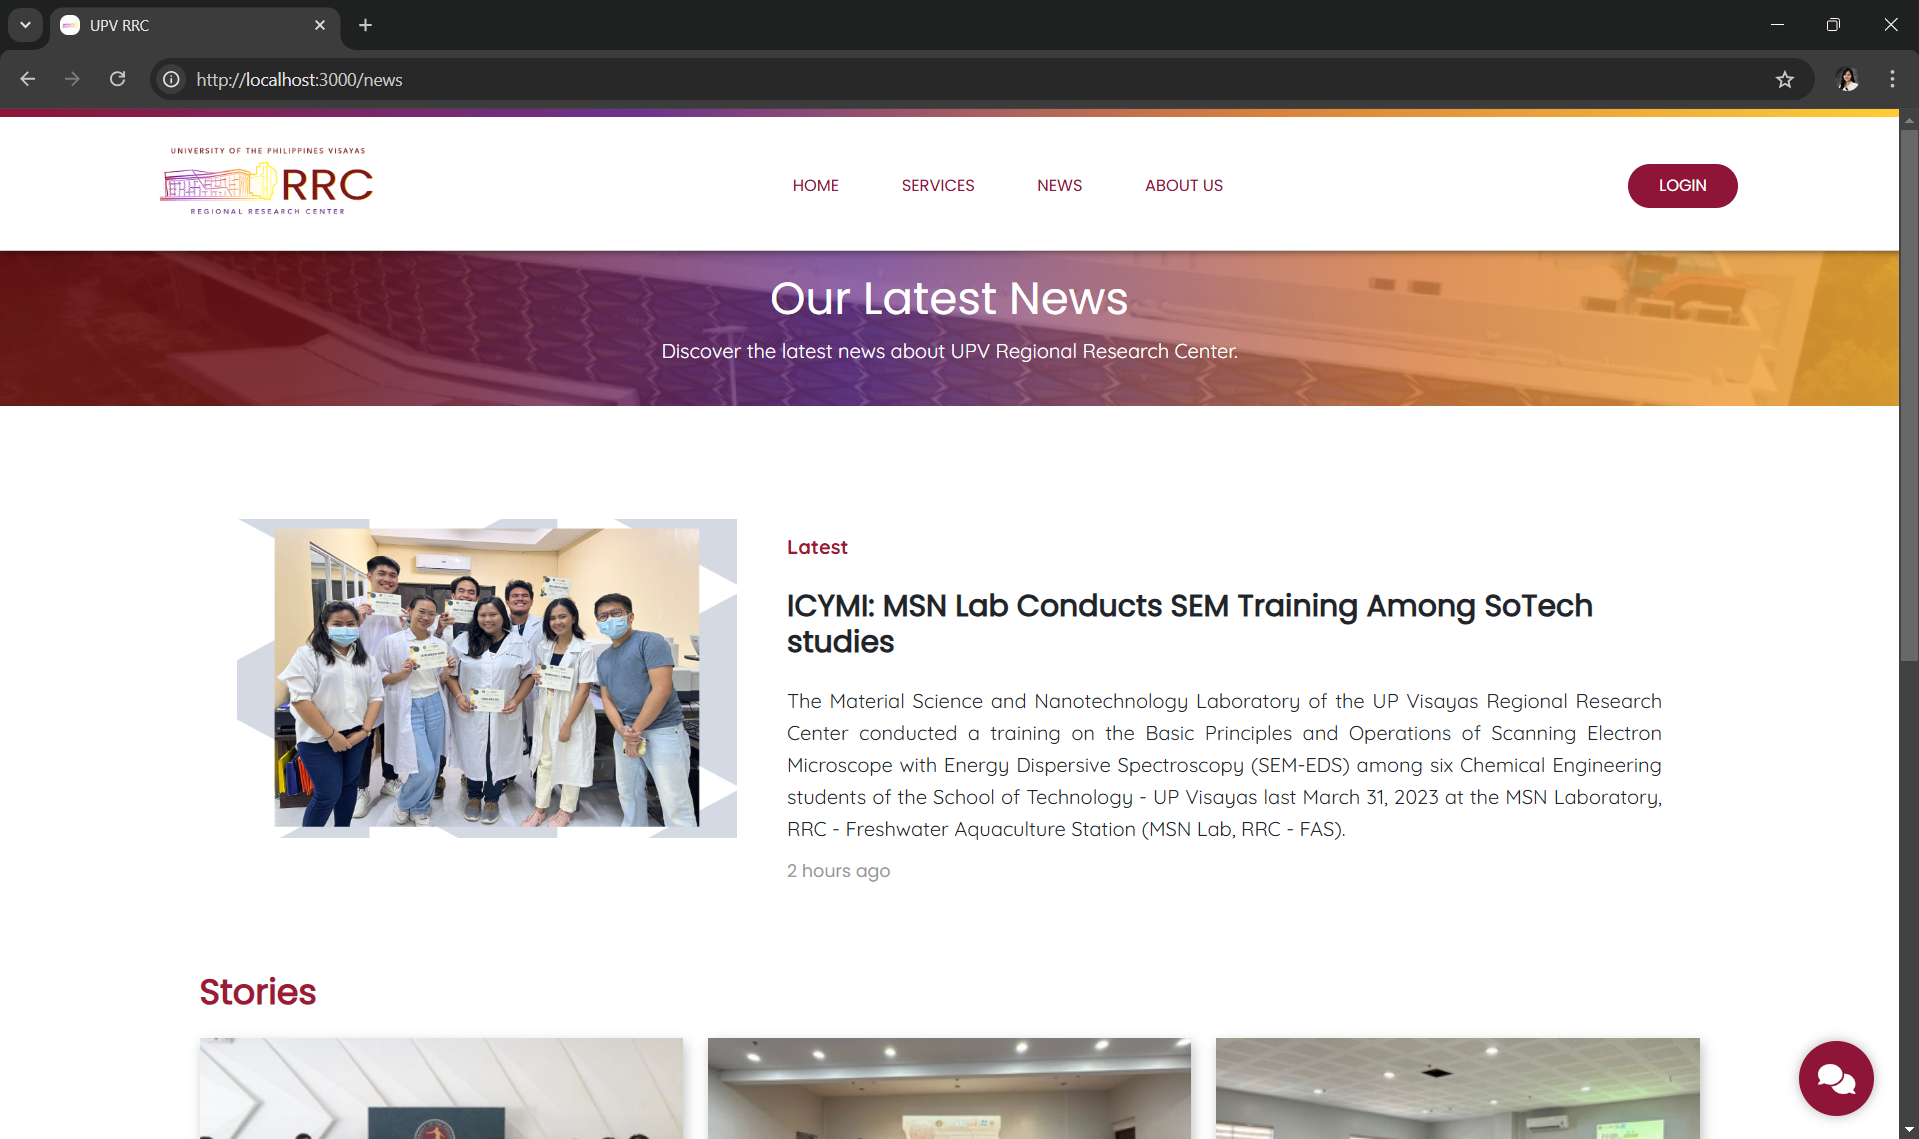
\includegraphics[width=0.8\textwidth]{news_page.png}
	\caption{News Page}
	\label{fig:news_page}
\end{figure}

\newpage

\noindent\textbf{About Us Page} 

Figure \ref{fig:about_page} shows the 'About Us' page. This page provides an overview of the RRC (Regional Research Center), detailing background information, its mission, vision, and team. It is designed to give visitors a deeper understanding of the organization and its role in the research community.

\begin{figure}[h]
	\centering
	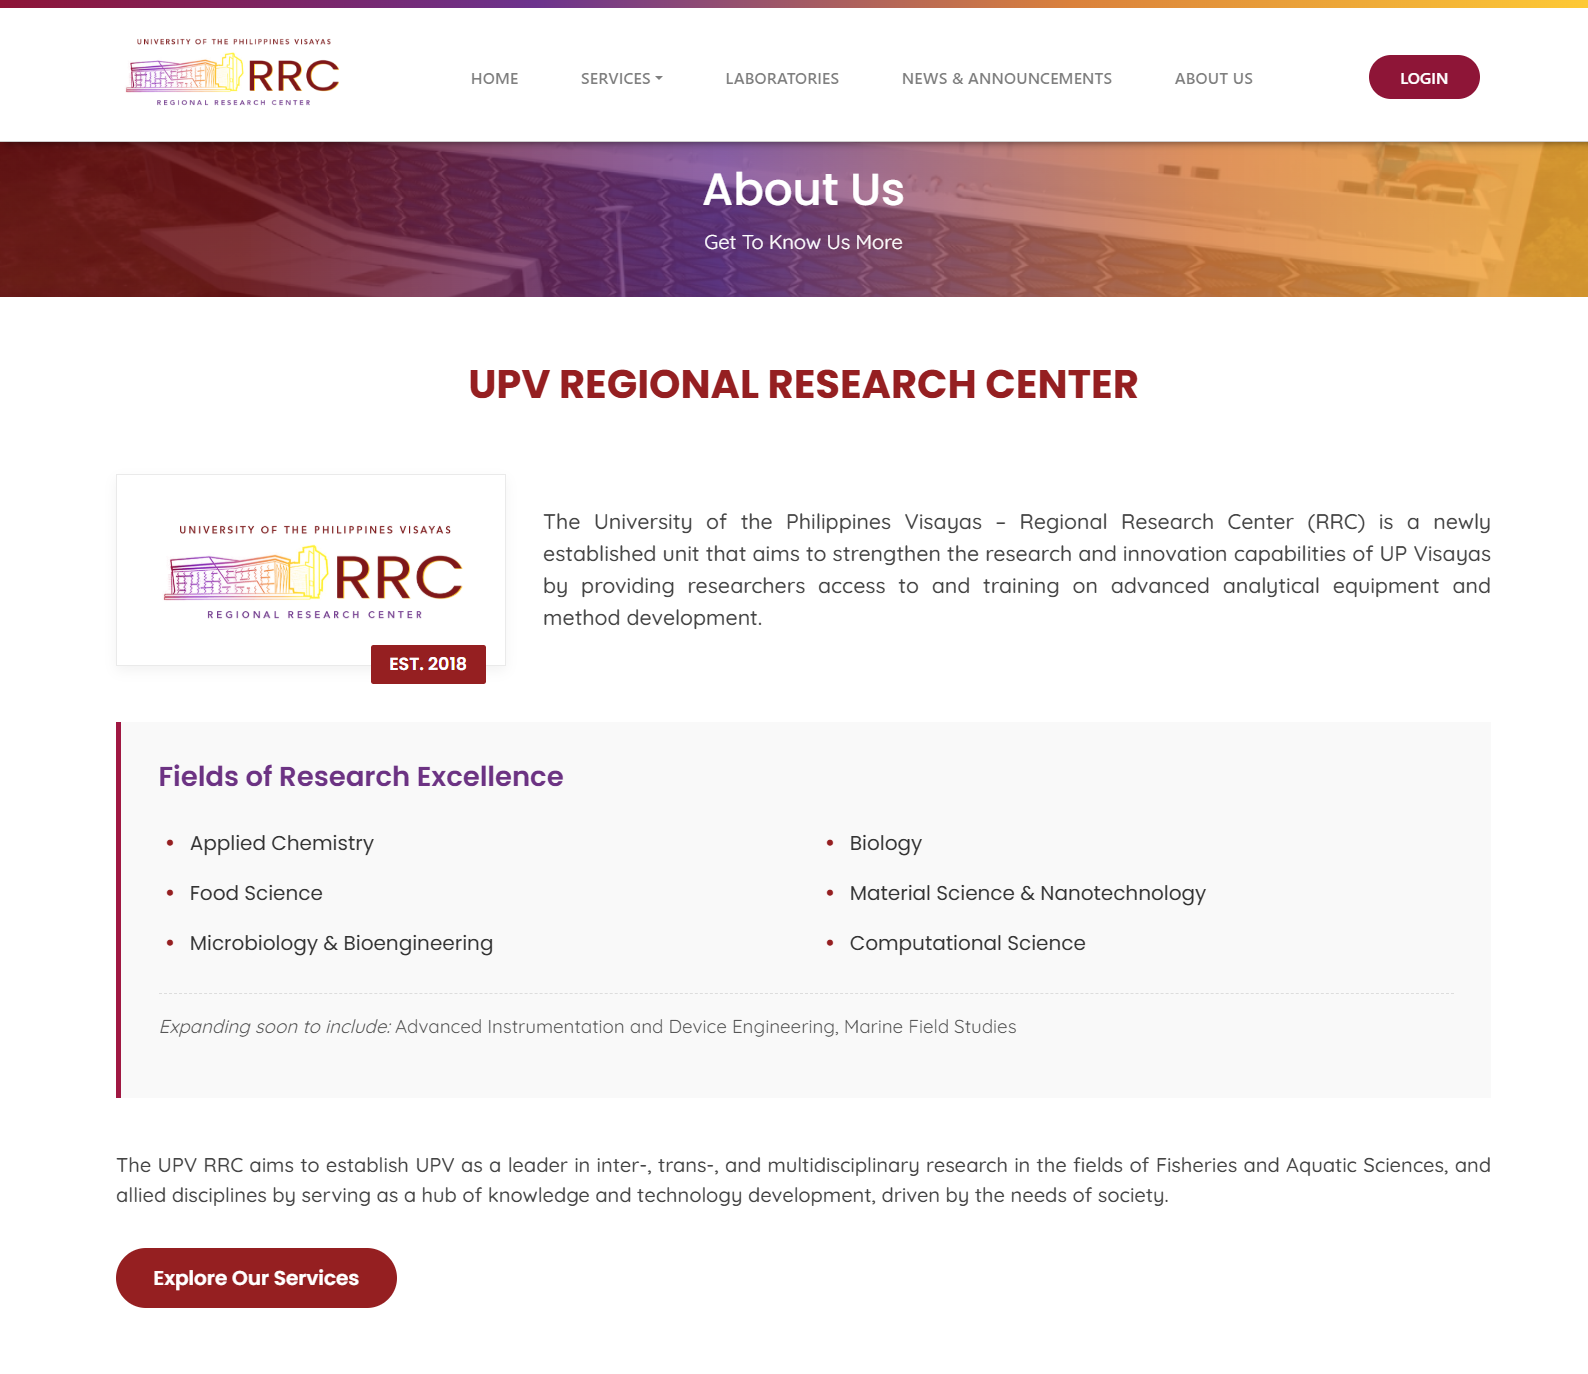
\includegraphics[width=0.8\textwidth]{about_page.png}
	\caption{About Page}
	\label{fig:about_page}
\end{figure}

\newpage

\subsection{Log in Module}

\noindent \textbf{User authentication}

Users can create their own accounts. However, by default, these accounts will remain inactive until the Admin Staff approves them after reviewing the user information. For clients, an additional step is required in which they must undergo an initial consultation with the staff. Only after this consultation will their account be permitted to submit a service request. This process ensures that new clients are informed about the proper procedures for requesting a service, as consultation is a necessary step.

On the login page, users need to enter their email address and password. Additionally, Google authentication is available, allowing users to sign in using their Google account for a quicker and more secure login experience. Passwords are hidden by default, but users can click the eye icon in the password field (as shown in \figref{fig:login}) to toggle visibility. After successfully logging in, users will be redirected to their respective dashboards.

\begin{figure}[h]
	\centering
	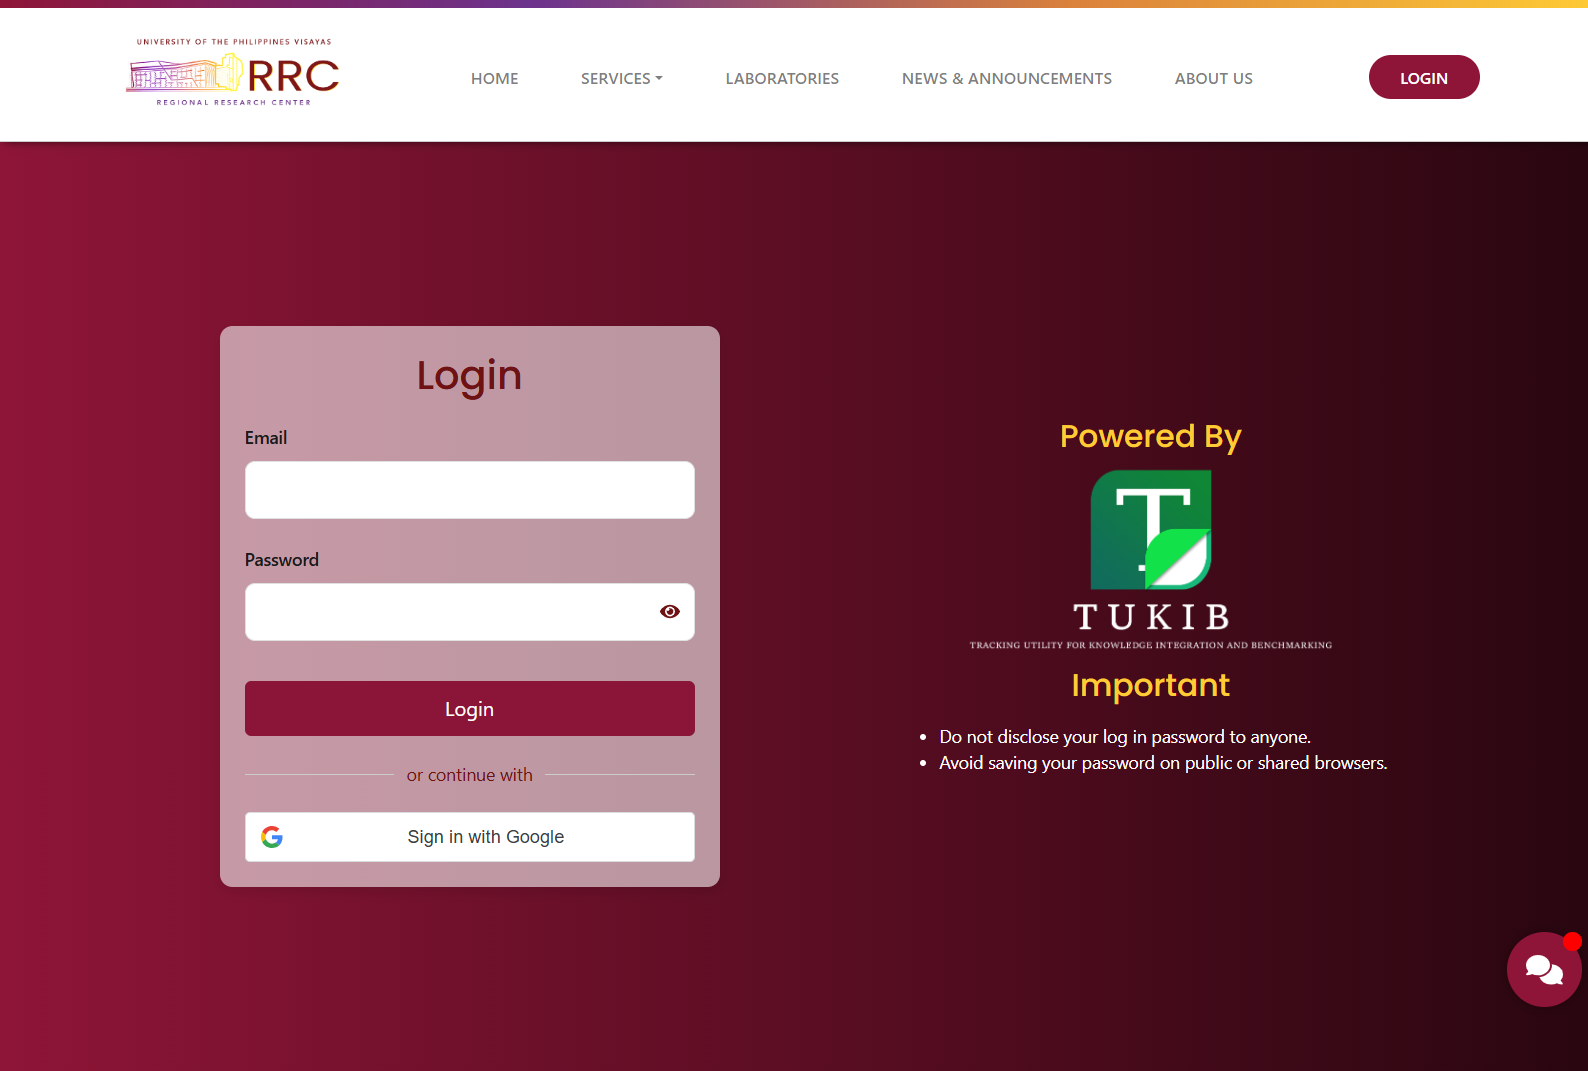
\includegraphics[width=0.80\textwidth]{login.png}
	\caption{Log in page}
	\label{fig:login}
\end{figure}

\noindent \textbf{User Dashboards}

User dashboard is designed for the needs of two primary user groups of TUKIB who are the staff and clients. Each user group has a different user interface to cater to their specific needs as seen from \figref{fig:client_dashboard} and \figref{fig:staff_dashboard}.

For the client’s account user interface, the developers designed a dashboard that shows the user’s profile, transaction history, and a button for availing a new service. For staff users, the interface is tailored to their specific responsibilities. For example, University Researchers are shown tools and information relevant to their assigned laboratories, including lab-specific service requests, equipments, and schedules. Admin Staff, on the other hand, have access to a comprehensive dashboard that allows them to oversee all service requests, approve accounts, manage workflows, and generate reports. This role-based design enhances efficiency by presenting only the relevant tools and information needed by each type of user.

\begin{figure}[h]
	\centering 
	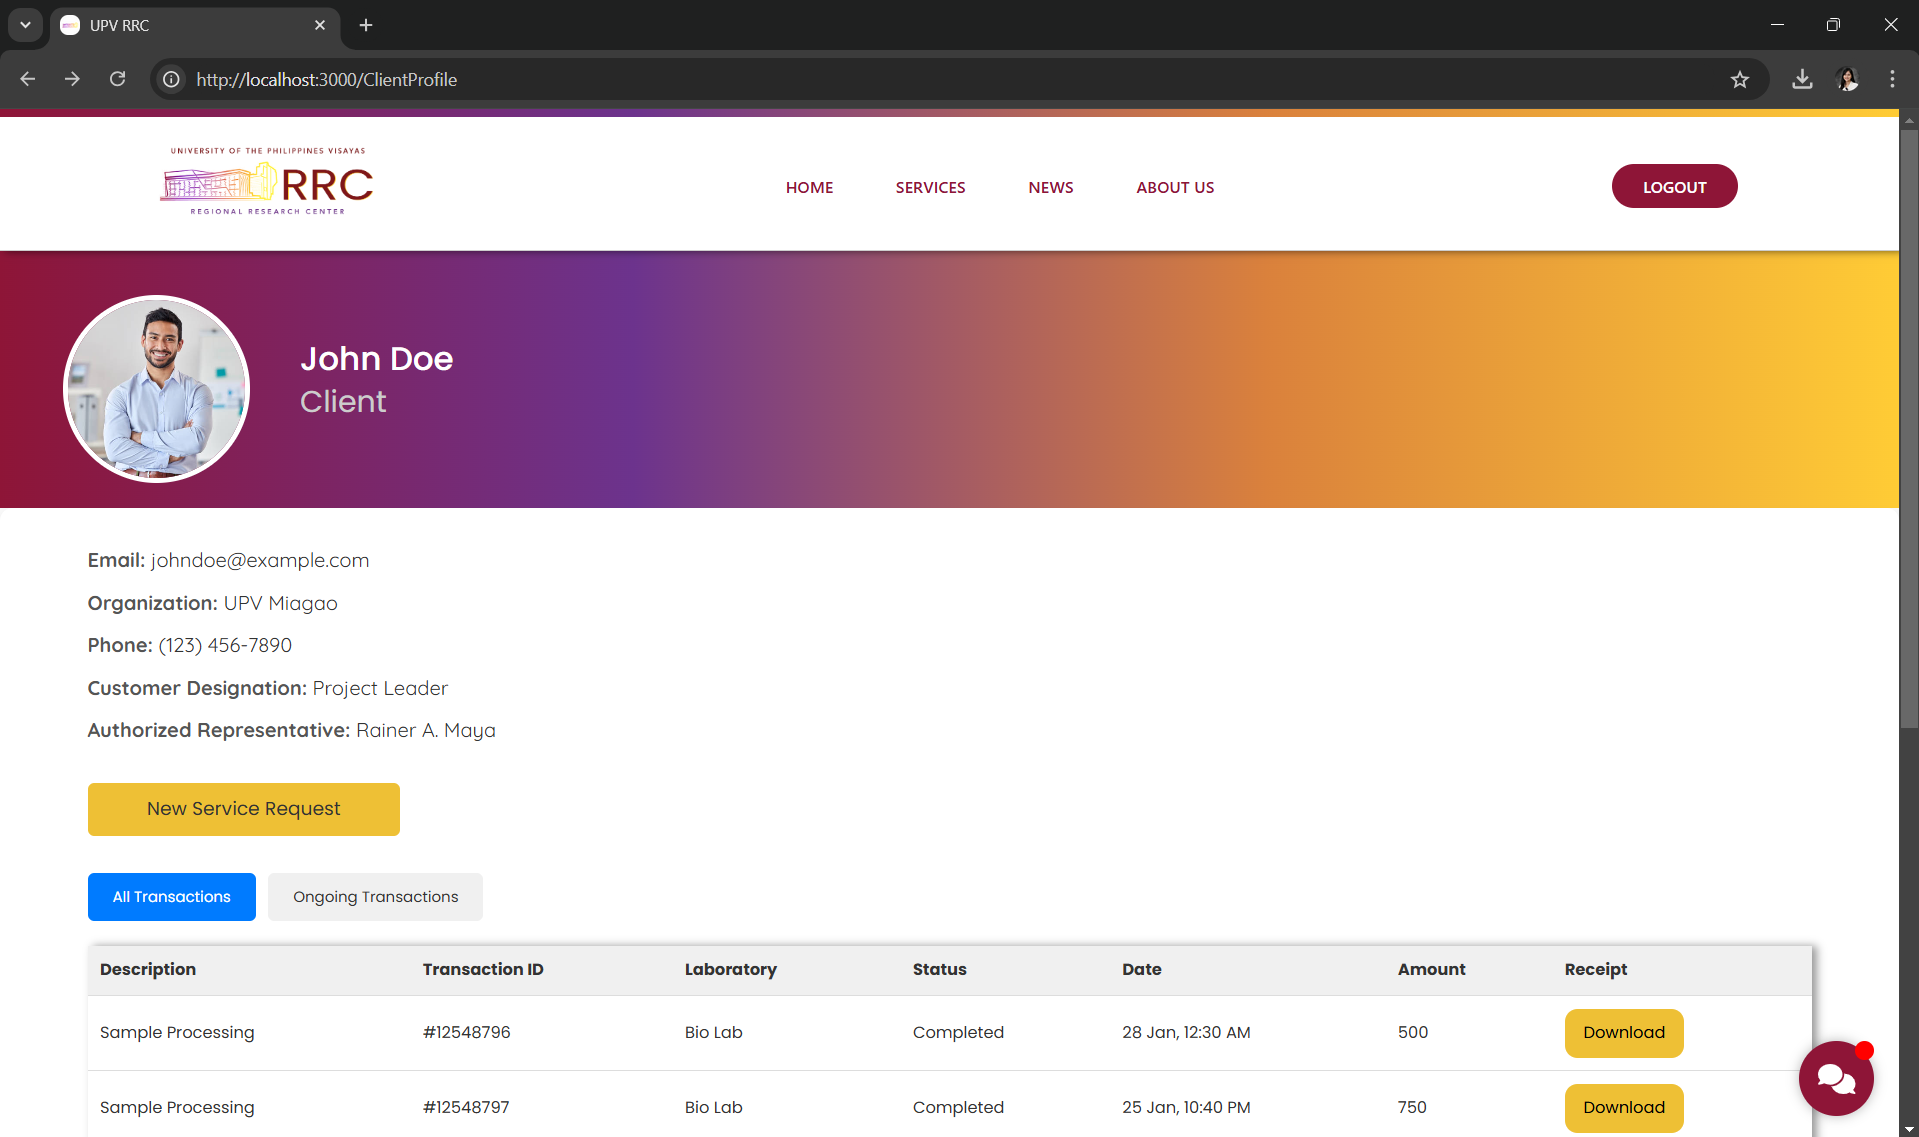
\includegraphics[width=0.8\textwidth]{client_dashboard.png}
	\caption{Client dashboard}
	\label{fig:client_dashboard}
\end{figure}

\newpage

\begin{figure}[h]
	\centering 
	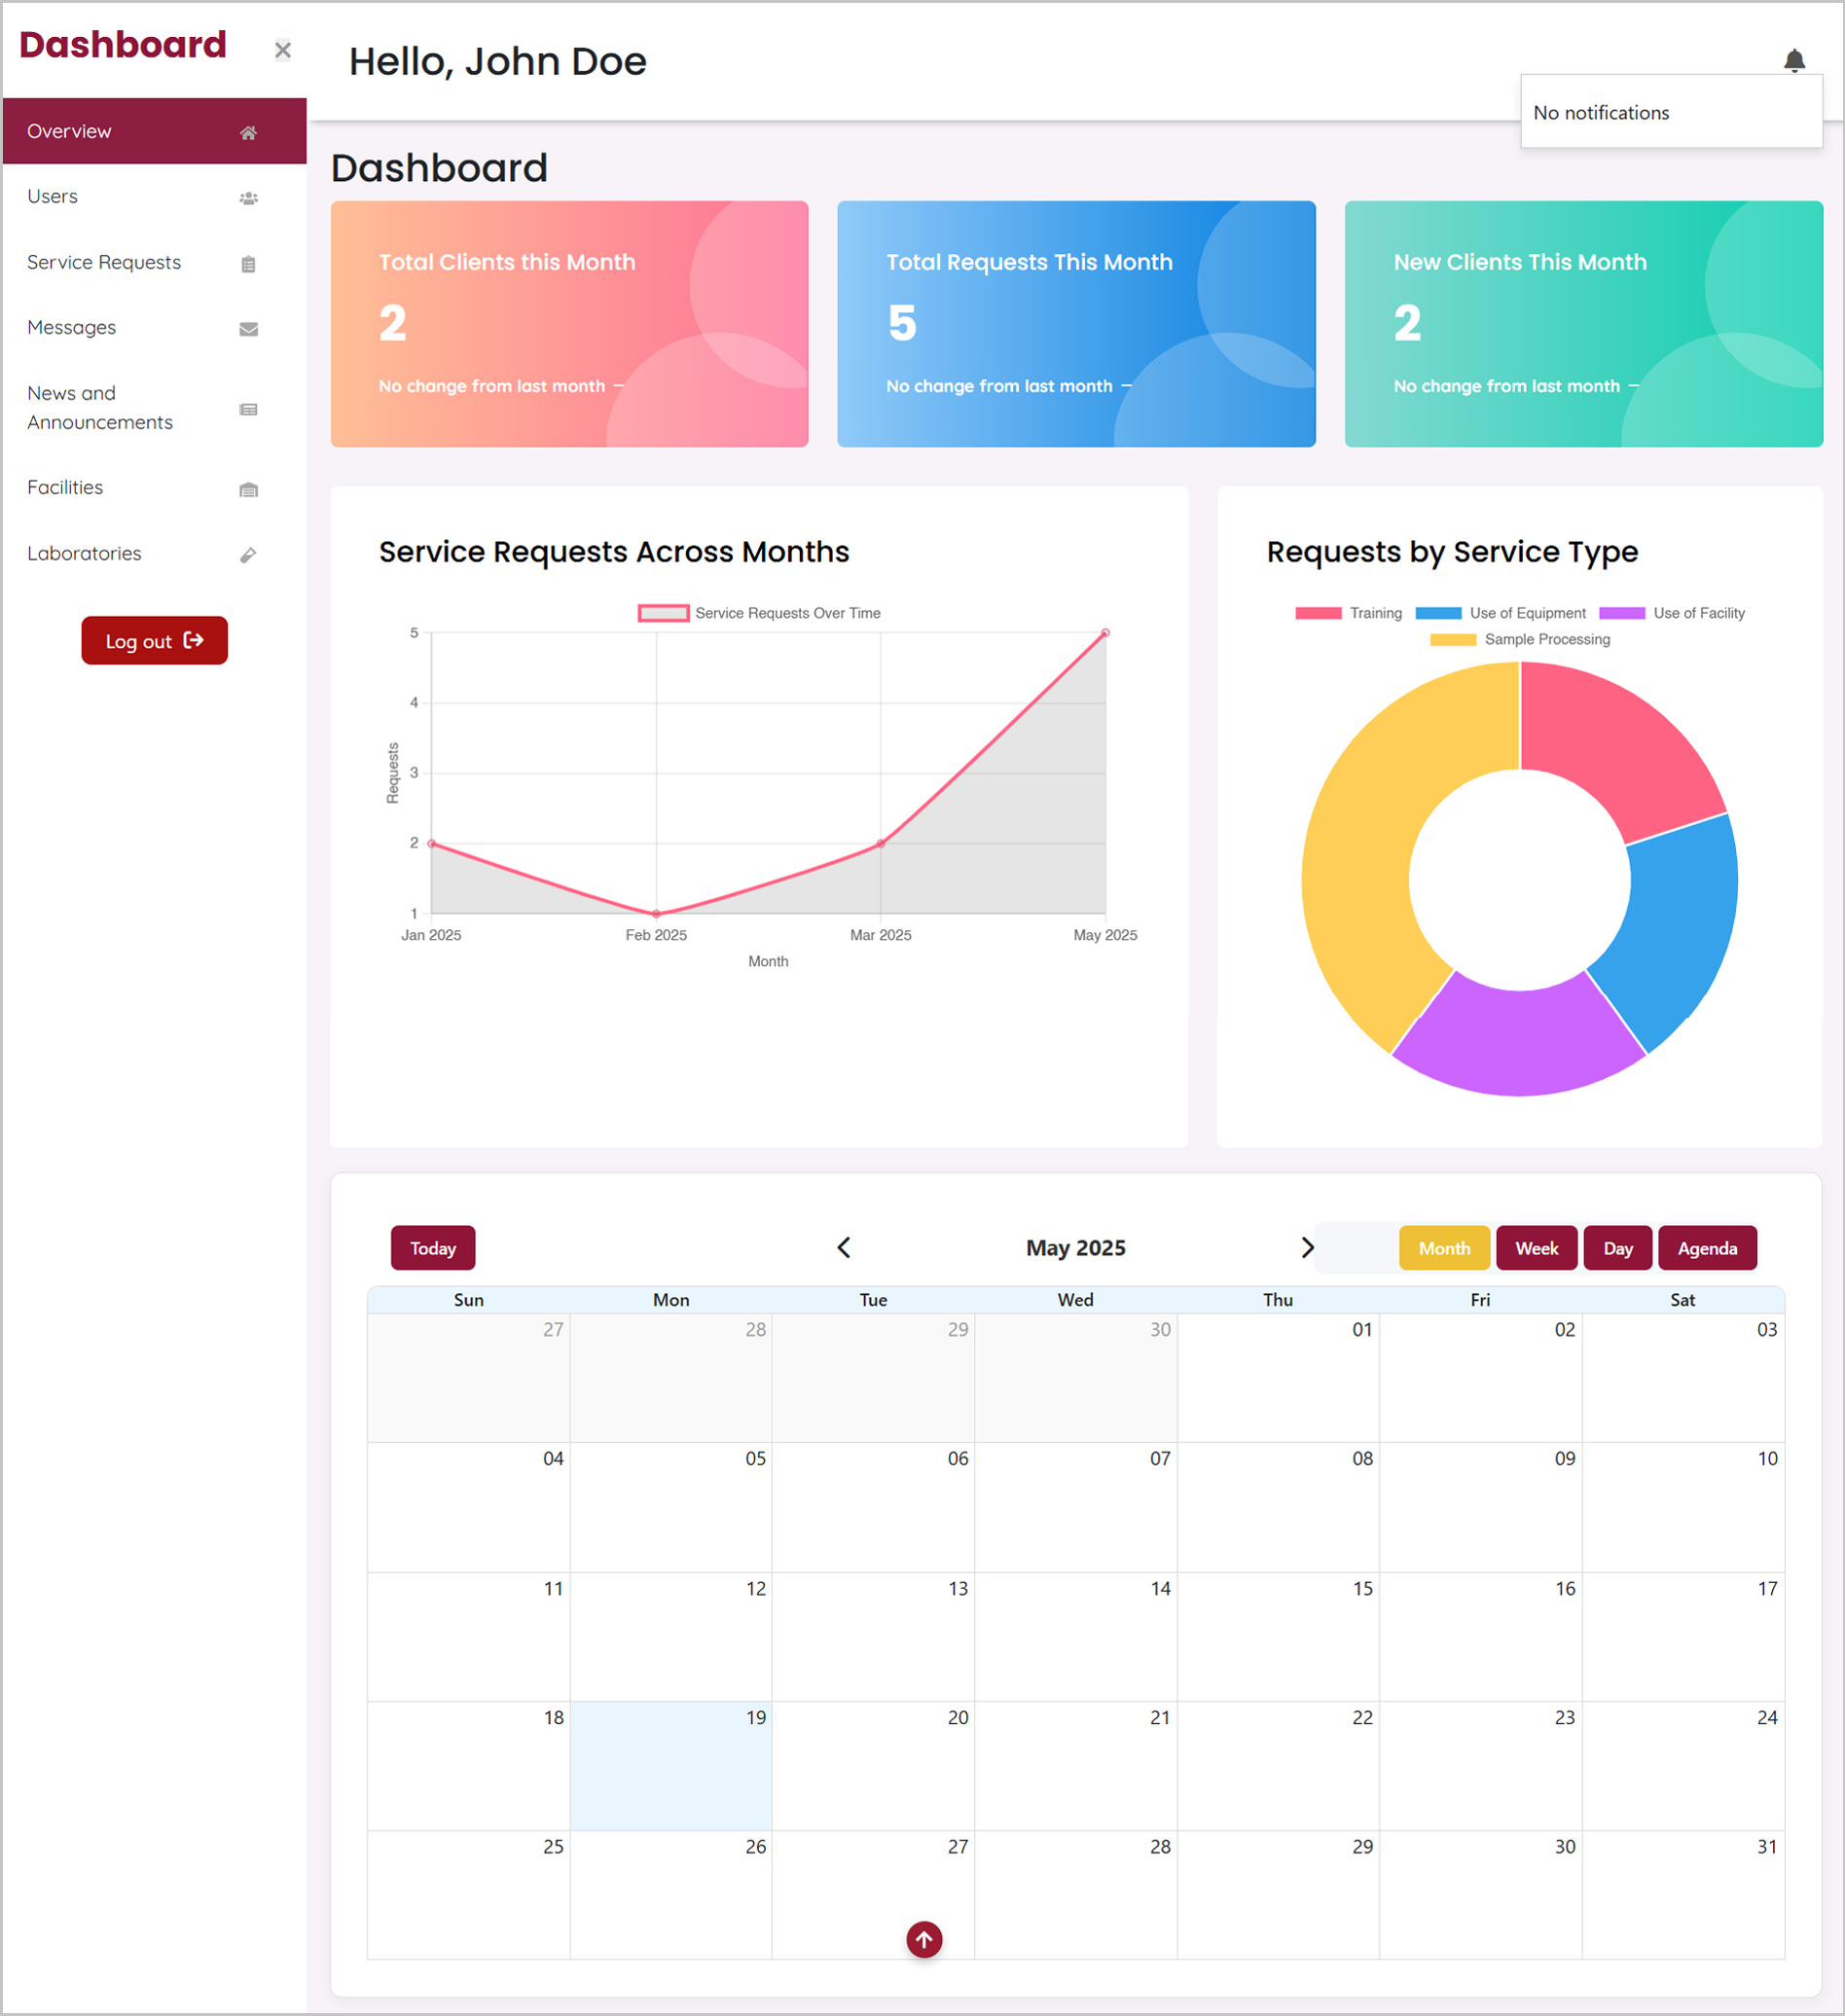
\includegraphics[width=0.8\textwidth]{staff_dashboard.png}
	\caption{Staff dashboard}
	\label{fig:staff_dashboard}
\end{figure}

\subsection{Service Request Module}

One of the core features of TUKIB is the Service Request Module, which allows clients and staffs to easily access, monitor, and manage service requests using their respective accounts. Clients are able to submit service requests, track statuses of requests, view results, upload payment receipt, and give feedback to the UPV RRC. On the other hand, staffs are able to approve or reject requests, update request statuses, upload charge slip and result, and view payment receipt from clients. This ensures that each request is processed efficiently from request to completion. 

Moreover, module guarantees that all data is centralized, providing a unified view of requests for better coordination among staffs and streamlined workflows. 

\subsection{Data Management Module}

Data management module is responsible for handling all the data within the system. This includes information of clients, transaction histories, inventory of equipment, and tracking of facility schedules and availability. This modules ensures that accounts are properly maintained while also allowing the staff to easily keep record of everything that is related to the RRC's service requests. It also streamlines the assignment of resources to users, maintains an up-to-date inventory, and provides a comprehensive view of resources, allowing for efficient allocation and tracking. Moreover, it enables staff and clients alike to view real time availability of equipment and facility, further guaranteeing the smooth and efficient flow of  service requests.

\section{Data Privacy and Security Measures}

\subsection{Password Encryption}

In order to ensure the security of user accounts, password hashing was implemented. This ensures that even if the database is compromised, plaintext passwords remain protected. The bcrypt algorithm was used due to its strength and resistance to brute-force attacks. Each password is hashed with a unique salt, which adds randomness and protects against rainbow table attacks.

During user registration, passwords are hashed before being stored in the database. During login, the hashed version of the input password is compared to the stored hash to authenticate users. This approach follows best practices in modern web security and ensures that sensitive credentials are never stored or transmitted in plain text.

\subsection{User Authentication and Authorization}

- Use of tokens (e.g., JWTs or sessions)
- Role-based access control (RBAC)
- Login attempt limits / account lockout

\subsection{Backup and Recovery}

include here:

- Secure backups
- Disaster recovery plans and frequency of testing

\section{Summary of Results}

To summarize the results of the study, the checklist of system requirements, Table \ref{tab:requirements}, was updated to indicate whether each requirement for TUKIB has been fulfilled. As shown in the Table \ref{tab:summary_results}, all of the system requirements have been successfully accomplished, demonstrating that the core functionalities of TUKIB are in place. However, a few areas still require further development or refinement to fully align with the intended specifications.

\begin{table}[ht]
	\centering
	\begin{tabular}{|p{10cm}|c|}
		\hline
		\textbf{Requirements/Modules} & \textbf{Accomplished (Y/N)} \\
		\hline
		\multicolumn{2}{|l|}{\textbf{Backend Requirements}} \\
		\hline
		Local Database & Y \\
		Automatic archiving & Y \\
		RESTful API & Y \\
		Role-based access control & Y \\
		Error handling, validation, \& logging & Y \\
		\hline
		\multicolumn{2}{|l|}{\textbf{Privacy Requirements}} \\
		\hline
		User password encryption & Y \\
		Session or token authentication & Y \\
		Restriction of unauthorized access & Y \\
		\hline
		\multicolumn{2}{|l|}{\textbf{User Interface Requirements}} \\
		\hline
		Client interface & Y \\
		Admin Staff interface & Y \\
		University Researcher interface & Y \\
		TECD Staff interface & Y \\
		Director interface & Y \\
		\hline
		\multicolumn{2}{|l|}{\textbf{Functional Requirements}} \\
		\hline
		User registration and authentication & Y \\
		Request tracking and management & Y \\
		Feedback mechanism & Y \\
		Notification system & Y \\
		Chatbot for FAQs and initial consultation & Y \\
		End-to-end flow of service request process & Y \\
		\hline
		\multicolumn{2}{|l|}{\textbf{UI/UX Design Requirements}} \\
		\hline
		Responsive design & Partially \\
		User-friendly navigation & Y \\
		Feedback/confirmation messages & Y \\
		\hline
	\end{tabular}
	\caption{System Requirements Checklist Result}
	\label{tab:summary_results}
\end{table}